\documentclass[11pt]{article}
\usepackage{amsmath}
\usepackage{amssymb}
\usepackage{bm}
\usepackage{algorithm}
\usepackage{algorithmic}
\usepackage{geometry}
\usepackage{tikz}
\usetikzlibrary{arrows.meta, positioning, decorations.pathreplacing}
\geometry{a4paper, margin=1in}

\title{SPAAL v2: Signal Processing Formulation}
\author{LiDAR Spoofing Attack Simulator}
\date{\today}

\begin{document}

\maketitle

\section{Overview}

This document formalizes the signal processing pipeline in SPAAL v2 (Simulator of the Physical Attack Against LiDARs), which models LiDAR measurements under High Frequency Radar (HFR) spoofing attacks.

The core data structure is a \textbf{3D signal tensor} (hist-matrix) $\bm{\mathcal{A}} \in \mathbb{R}^{C \times H \times T}$, where:
\begin{itemize}
    \item $C$: number of channels (vertical angles)
    \item $H$: horizontal resolution (azimuth samples)
    \item $T$: time bins (histogram length)
\end{itemize}

This tensor represents the composition of legitimate LiDAR returns and spoofing attack signals across all spatial and temporal dimensions.

\section{Time Coordinate Systems}

\subsection{Two Time Axes}

The system involves \textbf{two distinct time coordinate systems}:

\begin{enumerate}
    \item \textbf{Global time axis} $\tau \in \{0, 1, 2, \ldots, \tau_{\text{max}}-1\}$: Discrete absolute time (in nanoseconds) covering the entire LiDAR scan duration. The spoofer operates on this time axis. This time axis does \textbf{not} reset between measurements.

    \item \textbf{Local measurement time} $t \in \{0, 1, \ldots, T-1\}$: Discrete time bins for each individual measurement $(c, h)$, reset for every measurement. The hist-matrix uses this time axis.
\end{enumerate}

\textbf{Key difference}: Global time $\tau$ is continuous across the entire scan, while local time $t$ resets to 0 for each measurement $(c, h)$.

\subsection{Visual Representation of Time Axes}

\begin{figure}[h]
\centering
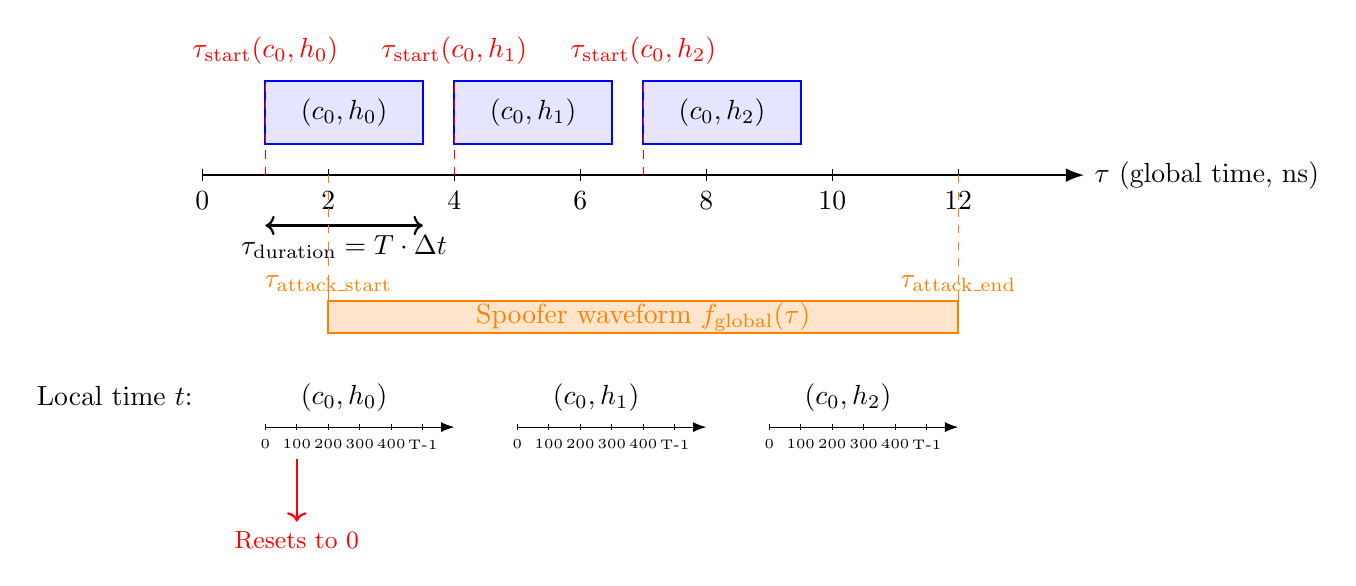
\begin{tikzpicture}[scale=0.8]
    % Global time axis
    \draw[-Latex, thick] (0,0) -- (14,0) node[right] {$\tau$ (global time, ns)};
    \foreach \x in {0,2,4,6,8,10,12}
        \draw (\x,0.1) -- (\x,-0.1) node[below] {\x};

    % Measurement windows
    \draw[thick, blue, fill=blue!10] (1,0.5) rectangle (3.5,1.5);
    \node at (2.25,1) {$(c_0, h_0)$};
    \draw[thick, blue, fill=blue!10] (4,0.5) rectangle (6.5,1.5);
    \node at (5.25,1) {$(c_0, h_1)$};
    \draw[thick, blue, fill=blue!10] (7,0.5) rectangle (9.5,1.5);
    \node at (8.25,1) {$(c_0, h_2)$};

    % tau_start markers
    \draw[dashed, red] (1,0) -- (1,1.5);
    \node[red, above] at (1,1.6) {$\tau_{\text{start}}(c_0, h_0)$};
    \draw[dashed, red] (4,0) -- (4,1.5);
    \node[red, above] at (4,1.6) {$\tau_{\text{start}}(c_0, h_1)$};
    \draw[dashed, red] (7,0) -- (7,1.5);
    \node[red, above] at (7,1.6) {$\tau_{\text{start}}(c_0, h_2)$};

    % tau_duration
    \draw[<->, thick] (1,-0.8) -- (3.5,-0.8);
    \node[below] at (2.25,-0.8) {$\tau_{\text{duration}} = T \cdot \Delta t$};

    % Spoofer continuous waveform
    \draw[thick, orange, fill=orange!20] (2,-2) rectangle (12,-2.5);
    \node[orange] at (7,-2.25) {Spoofer waveform $f_{\text{global}}(\tau)$};
    \draw[dashed, orange] (2,0) -- (2,-2);
    \draw[dashed, orange] (12,0) -- (12,-2);
    \node[orange, above] at (2,-2) {$\tau_{\text{attack\_start}}$};
    \node[orange, above] at (12,-2) {$\tau_{\text{attack\_end}}$};

    % Local time axes for each measurement
    \begin{scope}[yshift=-4cm]
        \node[left] at (0,0.5) {Local time $t$:};

        % Measurement (c0, h0)
        \draw[-Latex] (1,0) -- (4,0);
        \foreach \x/\label in {1/0, 1.5/100, 2/200, 2.5/300, 3/400, 3.5/T-1}
            \draw (\x,0.05) -- (\x,-0.05) node[below, font=\tiny] {\label};
        \node[above] at (2.25,0.1) {$(c_0, h_0)$};

        % Measurement (c0, h1)
        \draw[-Latex] (5,0) -- (8,0);
        \foreach \x/\label in {5/0, 5.5/100, 6/200, 6.5/300, 7/400, 7.5/T-1}
            \draw (\x,0.05) -- (\x,-0.05) node[below, font=\tiny] {\label};
        \node[above] at (6.25,0.1) {$(c_0, h_1)$};

        % Measurement (c0, h2)
        \draw[-Latex] (9,0) -- (12,0);
        \foreach \x/\label in {9/0, 9.5/100, 10/200, 10.5/300, 11/400, 11.5/T-1}
            \draw (\x,0.05) -- (\x,-0.05) node[below, font=\tiny] {\label};
        \node[above] at (10.25,0.1) {$(c_0, h_2)$};

        % Annotations
        \draw[thick, red, ->] (1.5,-0.5) -- (1.5,-1.5);
        \node[red, below] at (1.5,-1.5) {\small Resets to 0};
    \end{scope}
\end{tikzpicture}
\caption{Illustration of global time $\tau$ (continuous across scan) vs. local time $t$ (resets per measurement). The spoofer operates on global time and does not reset between measurements, while each LiDAR measurement window uses local time starting from 0.}
\end{figure}

\subsection{Mapping Between Time Axes}

Each measurement $(c, h)$ has a global start time $\tau_{\text{start}}(c, h)$ and duration $\tau_{\text{duration}}$.

\textbf{Time resolution}: $\Delta t = 1.0$ ns (default, typically 0.5--2.0 ns).

The relationship between local and global time is:

\begin{equation}
\tau = \tau_{\text{start}}(c, h) + t \cdot \Delta t
\end{equation}

The measurement window in global time is:
\begin{equation}
\tau \in [\tau_{\text{start}}(c, h), \tau_{\text{start}}(c, h) + \tau_{\text{duration}})
\end{equation}

where $\tau_{\text{duration}} = T \cdot \Delta t$ is the histogram window length.

\subsection{Scan Pattern}

For rotating LiDARs, the global start time depends on the scan pattern:

\begin{equation}
\tau_{\text{start}}(c, h) = \tau_{\text{scan\_begin}} + h \cdot \tau_{\text{step}}
\end{equation}

where:
\begin{itemize}
    \item $\tau_{\text{scan\_begin}}$: start time of the current rotation
    \item $\tau_{\text{step}}$: time between consecutive azimuth measurements
    \item For HDL-64E with dual firing: channels fire in pairs at each azimuth
\end{itemize}

\section{Signal Composition Model}

\subsection{3D Tensor Representation}

The observed histogram signal is represented as a 3D tensor $\bm{\mathcal{A}} \in \mathbb{R}^{C \times H \times T}$ (hist-matrix), which is the composition of legitimate LiDAR returns $\bm{\mathcal{L}} \in \mathbb{R}^{C \times H \times T}$ and spoofing signals $\bm{\mathcal{F}} \in \mathbb{R}^{C \times H \times T}$:

\begin{equation}
\bm{\mathcal{A}} = \bm{\mathcal{L}} + \bm{\mathcal{F}}(\bm{\mathcal{L}}) + \bm{\mathcal{N}}
\end{equation}

In element-wise notation:

\begin{equation}
\mathcal{A}(c, h, t) = \mathcal{L}(c, h, t) + \mathcal{F}(c, h, t \mid \mathcal{L}) + \mathcal{N}(c, h, t)
\end{equation}

\textbf{Note}: The spoofing signal $\bm{\mathcal{F}}$ is a function of $\bm{\mathcal{L}}$ for adaptive attacks, because the spoofer synchronizes its attack timing with the LiDAR's scan pattern and ToF measurements (detailed in Section 5).

where the tensor dimensions are:
\begin{itemize}
    \item $c \in \{0, 1, \ldots, C-1\}$: \textbf{channel index} (vertical angle, altitude)
    \item $h \in \{0, 1, \ldots, H-1\}$: \textbf{horizontal resolution index} (azimuth)
    \item $t \in \{0, 1, \ldots, T-1\}$: \textbf{time sample index} (histogram bins)
\end{itemize}

and the signal components are:
\begin{itemize}
    \item $\bm{\mathcal{A}} \in \mathbb{R}^{C \times H \times T}$: observed signal tensor (hist-matrix)
    \item $\bm{\mathcal{L}} \in \mathbb{R}^{C \times H \times T}$: legitimate LiDAR return tensor
    \item $\bm{\mathcal{F}} \in \mathbb{R}^{C \times H \times T}$: spoofing attack signal tensor
    \item $\bm{\mathcal{N}} \in \mathbb{R}^{C \times H \times T}$: environmental noise tensor (thermal, sunlight, etc.)
\end{itemize}

\subsection{Tensor Shape Parameters}

Typical tensor dimensions for different LiDAR models:
\begin{itemize}
    \item \textbf{HDL-64E}: $C = 64$ channels, $H = 4400$ (at 0.0818° resolution), $T = 1000\sim5000$ time bins
    \item \textbf{VLP-32c}: $C = 32$ channels, $H = 1800$ (at 0.2° resolution), $T = 1000\sim5000$ time bins
    \item \textbf{VLP-16}: $C = 16$ channels, $H = 1800$ (at 0.2° resolution), $T = 1000\sim5000$ time bins
\end{itemize}

\section{LiDAR Signal Model}

\subsection{Pulse Shape Function}

Both LiDAR and spoofer signals use a pulse shape function $p(t)$ to model the temporal profile of laser pulses. The standard model is a \textbf{Gaussian pulse}:

\begin{equation}
p(t) = \exp\left(-\frac{t^2}{2\sigma^2}\right)
\end{equation}

where the pulse width parameter $\sigma$ is related to the Full Width at Half Maximum (FWHM) by:

\begin{equation}
\sigma = \frac{\text{FWHM}}{2\sqrt{2\ln 2}} \approx \frac{\text{FWHM}}{2.355}
\end{equation}

Typical FWHM values:
\begin{itemize}
    \item LiDAR pulse: 5--10 ns
    \item Spoofer pulse: 3--10 ns
\end{itemize}

The pulse is typically computed over a finite support $t \in [-3\sigma, 3\sigma]$ (covering 99.7\% of the pulse energy).

\subsection{Pulse Generation}

The legitimate LiDAR return signal tensor $\bm{\mathcal{L}}$ is constructed by placing pulses at appropriate time bins. For each measurement $(c, h)$, a single pulse is modeled as:

\begin{equation}
\mathcal{L}(c, h, t) = A_{\text{pulse}}(c, h) \cdot p(t - t_{\text{ToF}}(c, h))
\end{equation}

where:
\begin{itemize}
    \item $A_{\text{pulse}}(c, h)$: pulse amplitude derived from target reflectivity at $(c, h)$
    \item $t_{\text{ToF}}(c, h)$: time-of-flight to the target at $(c, h)$ \textbf{in local time bins}
    \item $p(t)$: Gaussian pulse shape function (defined above)
\end{itemize}

\textbf{Note}: The LiDAR signal uses \textbf{local measurement time} $t$, reset for each measurement. This is different from the spoofer's global time $\tau$. The time-of-flight $t_{\text{ToF}}(c, h)$ is measured from the start of each measurement window, not from a global reference.

\subsection{Amplitude from Intensity}

For point cloud data with intensity $I \in [0, 1]$:

\begin{equation}
A_{\text{pulse}} = \begin{cases}
I \cdot \alpha & \text{if } I > 0 \\
0.05 \cdot \alpha & \text{if } I = 0
\end{cases}
\end{equation}

where $\alpha = 12.0$ is the intensity-to-amplitude conversion ratio. The default value $0.05$ prevents zero-intensity points from being filtered out.

\subsection{Time-of-Flight}

The true ToF is computed from target distance $d$ (in meters):

\begin{equation}
t_{\text{ToF}} = \frac{2d}{c_0 \cdot \Delta t}
\end{equation}

where $c_0 = 3 \times 10^8$ m/s is the speed of light. Factor of 2 accounts for round-trip travel.

For $\Delta t = 1.0$ ns, this simplifies to:
\begin{equation}
t_{\text{ToF}} = \frac{d}{0.15} \quad \text{(in time bins)}
\end{equation}

\section{Spoofer Signal Model}

The spoofing signal tensor $\bm{\mathcal{F}} \in \mathbb{R}^{C \times H \times T}$ represents malicious laser pulses injected by an attacker.

\subsection{Global Spoofing Waveform}

\textbf{Key concept}: The spoofer operates on the \textbf{global time axis} $\tau$ and generates an attack waveform $f_{\text{global}}(\tau)$ over the entire attack duration:

\begin{equation}
f_{\text{global}}(\tau): \{0, 1, \ldots, \tau_{\text{attack\_duration}}-1\} \rightarrow \mathbb{R}
\end{equation}

This global waveform does \textbf{not} reset between measurements—it persists across the entire LiDAR scan.

\subsection{Projection to Local Time}

The hist-matrix element $\mathcal{F}(c, h, t)$ is obtained by \textbf{sampling} the global waveform during the measurement window of $(c, h)$:

\begin{equation}
\mathcal{F}(c, h, t) = f_{\text{global}}(\tau_{\text{start}}(c, h) + t \cdot \Delta t)
\end{equation}

This represents the spoofer signal captured by the LiDAR during its measurement of direction $(c, h)$ at local time bin $t$.

\subsection{Timing Dependency}

\textbf{Important}: For adaptive attacks, $f_{\text{global}}(\tau)$ depends on the LiDAR scan timing and the legitimate signal $\bm{\mathcal{L}}$:

\begin{equation}
f_{\text{global}}(\tau) = f_{\text{global}}(\tau \mid \bm{\mathcal{L}}, \{\tau_{\text{start}}(c, h)\})
\end{equation}

This dependency arises because:
\begin{itemize}
    \item The spoofer knows when the LiDAR is measuring each direction $(c, h)$ via $\tau_{\text{start}}(c, h)$
    \item The attack timing can be chosen based on $t_{\text{ToF}}(c, h)$ from $\bm{\mathcal{L}}$
    \item The spoofer adapts its pulse train to interfere with specific measurements
\end{itemize}

\subsection{Adaptive HFR Attack}

The adaptive high-frequency radar (HFR) attack generates a periodic pulse train on the \textbf{global time axis}:

\begin{equation}
f_{\text{global}}(\tau \mid \bm{\mathcal{L}}) = \sum_{k \in \mathcal{K}} A_{\text{spoof}} \cdot p(\tau - \tau_k)
\end{equation}

where:
\begin{itemize}
    \item $\mathcal{K}$: set of pulse indices covering the attack duration
    \item $A_{\text{spoof}}$: spoofing pulse amplitude (typically 9.0)
    \item $\tau_k = \tau_{\text{attack\_start}} + k \cdot \tau_{\text{period}}$: global timing of $k$-th spoof pulse
    \item $\tau_{\text{period}}$: period of the HFR attack in global time (high frequency, e.g., 1--10 MHz)
    \item $p(\tau)$: Gaussian pulse shape function (Section 4.1)
\end{itemize}

\textbf{Adaptive timing}: The attack start time $\tau_{\text{attack\_start}}$ can be chosen based on the first measurement's ToF:

\begin{equation}
\tau_{\text{attack\_start}} = \tau_{\text{start}}(0, 0) + t_{\text{ToF}}(0, 0) \cdot \Delta t + \delta_{\text{offset}}
\end{equation}

where $\delta_{\text{offset}}$ is a strategic offset (e.g., to place spoofed points before/after true points).

The corresponding hist-matrix element is:

\begin{equation}
\mathcal{F}(c, h, t) = f_{\text{global}}(\tau_{\text{start}}(c, h) + t \cdot \Delta t)
\end{equation}

\subsection{Adaptive HFR with Perturbation}

Adding timing perturbation to evade simple filtering:

\begin{equation}
f_{\text{global}}(\tau \mid \bm{\mathcal{L}}) = \sum_{k \in \mathcal{K}} A_{\text{spoof}} \cdot p(\tau - \tau_k - \epsilon_k)
\end{equation}

where:
\begin{itemize}
    \item $\epsilon_k \sim \mathcal{N}(0, \sigma^2_{\text{perturb}})$: Gaussian timing jitter in global time (e.g., $\sigma_{\text{perturb}} = 1$--5 ns)
    \item $\tau_k = \tau_{\text{attack\_start}} + k \cdot \tau_{\text{period}}$ (base timing, before perturbation)
    \item $p(\tau)$: Gaussian pulse shape function (Section 4.1)
\end{itemize}

This makes the attack harder to detect via simple periodic pattern matching. The hist-matrix element is:

\begin{equation}
\mathcal{F}(c, h, t) = f_{\text{global}}(\tau_{\text{start}}(c, h) + t \cdot \Delta t)
\end{equation}

\subsection{Continuous Pulse Attack}

For continuous pulse spoofing, the global waveform is constant over the attack duration:

\begin{equation}
f_{\text{global}}(\tau) = \begin{cases}
A_{\text{continuous}} & \text{if } \tau \in [\tau_{\text{attack\_start}}, \tau_{\text{attack\_end}}) \\
0 & \text{otherwise}
\end{cases}
\end{equation}

where $\tau_{\text{attack\_start}}$ and $\tau_{\text{attack\_end}}$ define the attack window in global time.

The corresponding hist-matrix element is:

\begin{equation}
\mathcal{F}(c, h, t) = f_{\text{global}}(\tau_{\text{start}}(c, h) + t \cdot \Delta t)
\end{equation}

\textbf{Note}: Unlike adaptive attacks, continuous pulse does not depend on $\bm{\mathcal{L}}$'s ToF—only on the attack duration window. However, it still depends on scan timing $\{\tau_{\text{start}}(c, h)\}$ to map the global waveform to each measurement's local time.

\section{Peak Detection Algorithm}

This section describes how to extract distance and intensity from the observed signal tensor $\bm{\mathcal{A}}$. The algorithm processes each measurement $(c, h)$ independently by analyzing the 1D time-series signal $\mathcal{A}(c, h, \cdot)$.

\subsection{Pulse Rising Edge Detection}

For a fixed measurement $(c, h)$, detect pulse start indices where signal crosses threshold $\tau = 0.01$:

\begin{equation}
R(c, h) = \{t \mid \mathcal{A}(c, h, t-1) < \tau \text{ and } \mathcal{A}(c, h, t) \geq \tau\}
\end{equation}

\subsection{Peak Amplitude Search}

For each rising edge $r \in R(c, h)$, find maximum amplitude within search window $W = 50$ samples:

\begin{equation}
P_r(c, h) = \max_{t \in [r, r+W)} \mathcal{A}(c, h, t)
\end{equation}

\subsection{Strongest Pulse Selection}

Select the pulse with highest amplitude:

\begin{equation}
r^*(c, h) = \underset{r \in R(c, h)}{\arg\max} \; P_r(c, h)
\end{equation}

\begin{equation}
A_{\text{peak}}(c, h) = P_{r^*(c,h)}(c, h)
\end{equation}

\subsection{Parabolic Interpolation}

Find integer peak index within the selected pulse:

\begin{equation}
t_{\text{peak}}(c, h) = r^*(c, h) + \underset{t \in [r^*(c,h), r^*(c,h)+W)}{\arg\max} \; \mathcal{A}(c, h, t)
\end{equation}

Apply logarithmic parabolic interpolation using three neighboring samples:

\begin{equation}
y_{-1} = \mathcal{A}(c, h, t_{\text{peak}}-1), \quad y_0 = \mathcal{A}(c, h, t_{\text{peak}}), \quad y_1 = \mathcal{A}(c, h, t_{\text{peak}}+1)
\end{equation}

If $y_{-1}, y_0, y_1 > 0$, compute log values:

\begin{equation}
\ln y_{-1}, \quad \ln y_0, \quad \ln y_1
\end{equation}

Compute sub-sample offset $\delta$:

\begin{equation}
\delta = \frac{\ln y_{-1} - \ln y_1}{2(\ln y_{-1} - 2\ln y_0 + \ln y_1)}
\end{equation}

provided that $|\ln y_{-1} - 2\ln y_0 + \ln y_1| > 10^{-9}$.

The interpolated peak time is:

\begin{equation}
t_{\text{peak}}^{\text{interp}} = t_{\text{peak}} + \delta
\end{equation}

\subsection{Distance Reconstruction}

Convert interpolated time to distance:

\begin{equation}
d_{\text{recon}} = t_{\text{peak}}^{\text{interp}} \cdot \Delta t \cdot 0.15 \quad \text{(meters)}
\end{equation}

\section{3D Point Reconstruction}

\subsection{Angular Coordinates}

For each measurement at channel $c$ and horizontal index $h$:

\begin{equation}
\theta_{\text{azimuth}}(h) = \frac{h}{H} \cdot \text{FOV} + \theta_{\text{offset}}
\end{equation}

\begin{equation}
\phi_{\text{altitude}}(c) = \text{vertical\_angles}[c]
\end{equation}

where:
\begin{itemize}
    \item FOV = 360° for full rotation LiDARs
    \item $\theta_{\text{offset}}$: initial azimuth offset
    \item vertical\_angles: LiDAR-specific channel angles
\end{itemize}

\subsection{Cartesian Coordinates}

Convert to 3D Cartesian coordinates:

\begin{equation}
\begin{aligned}
x &= d_{\text{recon}} \cdot \cos(\phi_{\text{altitude}}) \cdot \sin(\theta_{\text{azimuth}}) \\
y &= d_{\text{recon}} \cdot \cos(\phi_{\text{altitude}}) \cdot \cos(\theta_{\text{azimuth}}) \\
z &= d_{\text{recon}} \cdot \sin(\phi_{\text{altitude}})
\end{aligned}
\end{equation}

\subsection{Intensity Mapping}

The reconstructed intensity is:

\begin{equation}
I_{\text{recon}} = \min\left(A_{\text{peak}} \cdot \beta, 255\right)
\end{equation}

where $\beta$ is the amplitude-to-intensity ratio (default: $255/10 = 25.5$).

\section{Special Cases}

\subsection{No Valid Peak}

If any of the following conditions hold:
\begin{itemize}
    \item $R = \emptyset$ (no rising edges detected)
    \item $\max_r P_r < \tau$ (all peaks below threshold)
    \item Parabolic interpolation fails (denominator near zero)
\end{itemize}

then return:
\begin{equation}
t_{\text{peak}}^{\text{interp}} = 0, \quad A_{\text{peak}} = 0
\end{equation}

and exclude this measurement from the reconstructed point cloud.

\subsection{Answer Matrix (Ground Truth)}

For prediction/answer matrix format, the 3D tensor $\bm{\mathcal{A}}$ is reduced to a 2D matrix that directly stores peak times:

\begin{equation}
\bm{\mathcal{A}}_{\text{answer}} \in \mathbb{R}^{C \times H}
\end{equation}

where each element is:

\begin{equation}
\mathcal{A}_{\text{answer}}(c, h) = t_{\text{peak}}^{\text{interp}}(c, h)
\end{equation}

Note: The time dimension is collapsed by storing only the peak time (a scalar) for each measurement $(c, h)$.

Distance reconstruction uses the stored time directly without peak detection:

\begin{equation}
d_{\text{recon}}(c, h) = \mathcal{A}_{\text{answer}}(c, h) \cdot \Delta t \cdot 0.15
\end{equation}

\section{Summary of Parameters}

\subsection{Tensor Dimensions}

\begin{table}[h]
\centering
\begin{tabular}{|l|l|l|l|}
\hline
\textbf{LiDAR Model} & \textbf{Channels ($C$)} & \textbf{Azimuth ($H$)} & \textbf{Time Bins ($T$)} \\
\hline
HDL-64E & 64 & 4400 & 1000--5000 \\
VLP-32c & 32 & 1800 & 1000--5000 \\
VLP-16 & 16 & 1800 & 1000--5000 \\
\hline
\end{tabular}
\caption{Typical tensor dimensions for different LiDAR models}
\end{table}

\subsection{Algorithm Parameters}

\begin{table}[h]
\centering
\begin{tabular}{|l|l|l|}
\hline
\textbf{Parameter} & \textbf{Symbol} & \textbf{Default Value} \\
\hline
Detection threshold & $\tau$ & 0.01 \\
Peak search window & $W$ & 50 samples \\
Time resolution & $\Delta t$ & 1.0 ns \\
Speed of light factor & $c_0/2$ & 0.15 m/ns \\
Intensity-to-amplitude ratio & $\alpha$ & 12.0 \\
Amplitude-to-intensity ratio & $\beta$ & 25.5 \\
Default intensity (zero case) & - & 0.05 \\
Interpolation stability threshold & - & $10^{-9}$ \\
\hline
\end{tabular}
\caption{Key parameters in signal processing pipeline}
\end{table}

\section{Algorithm Summary}

\begin{algorithm}
\caption{Peak Detection and Distance Reconstruction from Tensor $\bm{\mathcal{A}}$}
\begin{algorithmic}[1]
\REQUIRE Observed signal tensor $\bm{\mathcal{A}} \in \mathbb{R}^{C \times H \times T}$, measurement $(c, h)$
\ENSURE Distance $d_{\text{recon}}(c, h)$, Intensity $I_{\text{recon}}(c, h)$
\STATE $R \gets \{t \mid \mathcal{A}(c,h,t-1) < 0.01 \land \mathcal{A}(c,h,t) \geq 0.01\}$
\IF{$R = \emptyset$}
    \RETURN $(0, 0)$
\ENDIF
\FOR{$r \in R$}
    \STATE $P_r \gets \max_{t \in [r, r+50)} \mathcal{A}(c, h, t)$
\ENDFOR
\STATE $r^* \gets \arg\max_r P_r$
\STATE $A_{\text{peak}} \gets P_{r^*}$
\IF{$A_{\text{peak}} < 0.01$}
    \RETURN $(0, 0)$
\ENDIF
\STATE $t_{\text{peak}} \gets r^* + \arg\max_{t \in [r^*, r^*+50)} \mathcal{A}(c, h, t)$
\STATE $y_{-1}, y_0, y_1 \gets \mathcal{A}(c, h, t_{\text{peak}}-1:t_{\text{peak}}+2)$
\IF{$y_{-1}, y_0, y_1 > 0$}
    \STATE $\delta \gets \frac{\ln y_{-1} - \ln y_1}{2(\ln y_{-1} - 2\ln y_0 + \ln y_1)}$
    \STATE $t_{\text{peak}}^{\text{interp}} \gets t_{\text{peak}} + \delta$
\ELSE
    \STATE $t_{\text{peak}}^{\text{interp}} \gets t_{\text{peak}}$
\ENDIF
\STATE $d_{\text{recon}}(c, h) \gets t_{\text{peak}}^{\text{interp}} \cdot 0.15$ (meters)
\STATE $I_{\text{recon}}(c, h) \gets \min(A_{\text{peak}} \cdot 25.5, 255)$
\RETURN $(d_{\text{recon}}(c, h), I_{\text{recon}}(c, h))$
\end{algorithmic}
\end{algorithm}

\subsection{Reconstruction for Full Tensor}

To reconstruct the complete point cloud from tensor $\bm{\mathcal{A}} \in \mathbb{R}^{C \times H \times T}$:

\begin{algorithm}
\caption{Full Point Cloud Reconstruction}
\begin{algorithmic}[1]
\REQUIRE Observed signal tensor $\bm{\mathcal{A}} \in \mathbb{R}^{C \times H \times T}$
\ENSURE Point cloud $\mathcal{P} = \{(x_i, y_i, z_i, I_i)\}$
\STATE $\mathcal{P} \gets \emptyset$
\FOR{$c = 0$ to $C-1$}
    \FOR{$h = 0$ to $H-1$}
        \STATE $(d, I) \gets \text{PeakDetection}(\bm{\mathcal{A}}, c, h)$ \COMMENT{Algorithm 1}
        \IF{$d > 0$}
            \STATE $(x, y, z) \gets \text{SphericalToCartesian}(c, h, d)$
            \STATE $\mathcal{P} \gets \mathcal{P} \cup \{(x, y, z, I)\}$
        \ENDIF
    \ENDFOR
\ENDFOR
\RETURN $\mathcal{P}$
\end{algorithmic}
\end{algorithm}

\end{document}
